


\documentclass[12pt]{article}

\setlength{\topmargin}{0pt}
\setlength{\textheight}{9in}
\setlength{\headheight}{0pt}
\setlength{\headsep}{0pt}
\setlength{\oddsidemargin}{0.25in}
\setlength{\textwidth}{6in}
\pagestyle{plain}
\usepackage{graphicx}
\graphicspath{ {./} }
\usepackage{amssymb}

\begin{document}

%\thispagestyle{empty}

%\raisebox{0.6in}[0in]{\makebox[\textwidth][r]{\it
% DRAFT --- a final version will be posted shortly}}
%\vspace{-0.7in}

\begin{center}
\bf\large CS 541: Artificial Intelligence
\end{center}

\noindent
Instructor: Jie Shen
\hfill
Lecture 9               %%% FILL IN LECTURE NUMBER HERE
\\
Scribe:   David Staronka and Omkar Sinha              %%% FILL IN YOUR NAME HERE
\hfill
November 9, 2021                         %%% FILL IN LECTURE DATE HERE

\noindent
\rule{\textwidth}{1pt}

\medskip

%%%%%%%%%%%%%%%%%%%%%%%%%%%%%%%%%%%%%%%%%%%%%%%%%%%%%%%%%%%%%%%%
%% BODY OF SCRIBE NOTES GOES HERE
%%%%%%%%%%%%%%%%%%%%%%%%%%%%%%%%%%%%%%%%%%%%%%%%%%%%%%%%%%%%%%%%

    \section{Deep Learning Model}
    A typical deep learning model is as follows:\\
    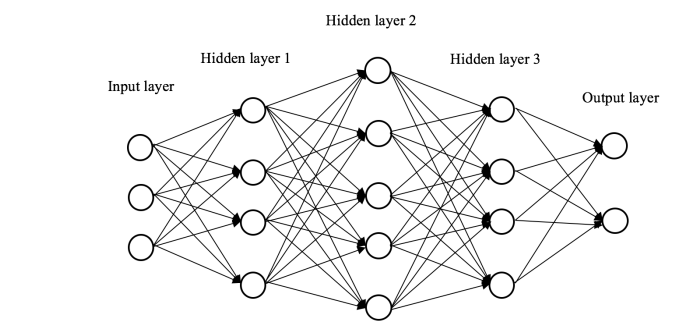
\includegraphics[scale=0.9]{2nd Scribe Notes/illustration.PNG}
    \\
    
    Here the Nodes are one of more weighted input connections and produce an output connection. They're organised into layers to comprise a network. Many such layers, together form a Neural Network, i.e. the foundation of Deep Learning.
    The input layer receives the input and the output layer produces results. 
    \\
    
    However the intermediate layers workings are not recognizable to us, and are called the hidden layers and together constitute the black box as follows:
    \\
    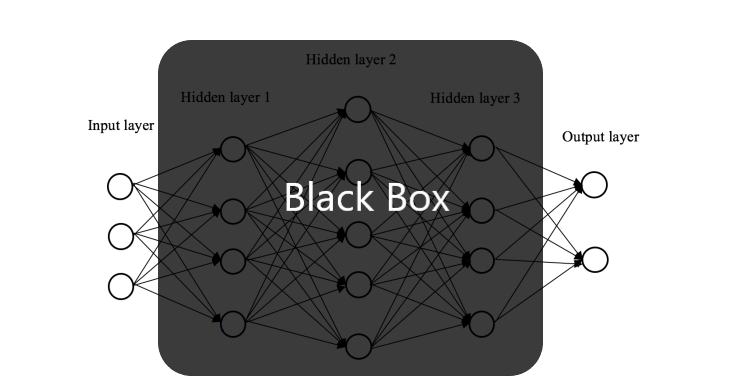
\includegraphics[scale=0.9]{2nd Scribe Notes/illustration2.PNG}
    \\
    \section{Optimization of Deep Learning Model}
    
    Since the model is like a black box it is challenging for us to effectively optimize. One way to optimize the model could be to simply increase the number of parameters, however such an approach will lead to increase in model complexity which will make it costlier to train. When we take the opposite approach, we face overfitting.\\
    
    So the question is how to find the optimum size of the model?
    \\
    We take one approach, where we recognize the overfitting to be caused by the model learning some extra features. We can use model compression to filter those nodes learning extra information. We can do this manually using techniques like node pruning or by using a function low rank factorization which uses matrix/tensor decomposition to project the initial d-dimension layer to lower rank compressed k-dimension layer.\\
    
    While this is helpful it has the possibility of us filtering out the important parameters. So now the question arises as how to develop a deep learning model which can itself determine which information is important or not.
    \section{Knowledge Distillation}
    A technique to develop a model that meets these requirement was proposed in 2015 by Geoffrey Hinton. This is called knowledge distillation which can also be called teacher-student model for simplicity. This has one complex 'teacher' model which well-trained in advance and the other smaller distilled student model.\\
    
    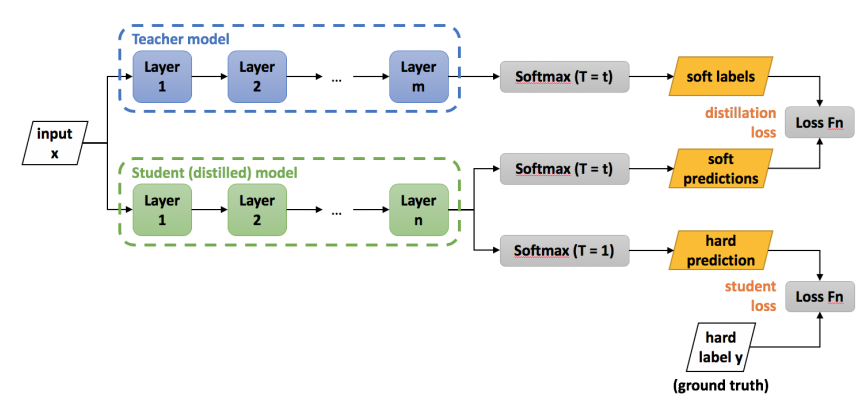
\includegraphics[scale=0.8]{2nd Scribe Notes/illustration3.PNG} 
    \\
    
    In the above knowledge distillation representation, the student model is trained by the comparing its output with that of the teacher model. Here we call the loss observed between the student  and teacher model as distillation loss. We also compare the 1st layer of the student model with ground truth and record the loss as student loss. The loss function ${\pounds}$ is given as: \\
    
    ${\pounds} = {\lambda}{\pounds}(f_t,f_s)+(1-{\lambda}){\pounds}(f_s,y)$\\
    \\where $f_s$ = outcome of student model, $f_t$ = outcome of teacher model and $y$ = ground truth\\
    
    The loss function is divided into two parts - the first student model learned from teacher and the second part shows student model learns from ground truth.\\
    
    \subsection{Response-based Knowledge:}
    
    According to the model proposed by Hinton, the knowledge is defined as the output of teacher model known as logits, which are also called response-based knowledge. Acc. to this the softmax is defined as follows: \\
    
    $p(x_i,T) = \frac{exp(x_i/T)}{\sum_j exp(x_j/T)} \rightarrow \pounds_{CE}(p(f_t(x),T),p(f_t(x),T))$ \\
    \\
    where, T is temperature or margin controller that depicts the relative values of the parameters:
    \\
    $0<t<1$ one factor is enhanced \\
    $t>1$ factors are similar \\
    when CE(cross-entrophy) = 0, student learns well from teacher model.\\
    
    An example of response based learning below shows the difference of image recognition between using hard label and soft label.\\
    
    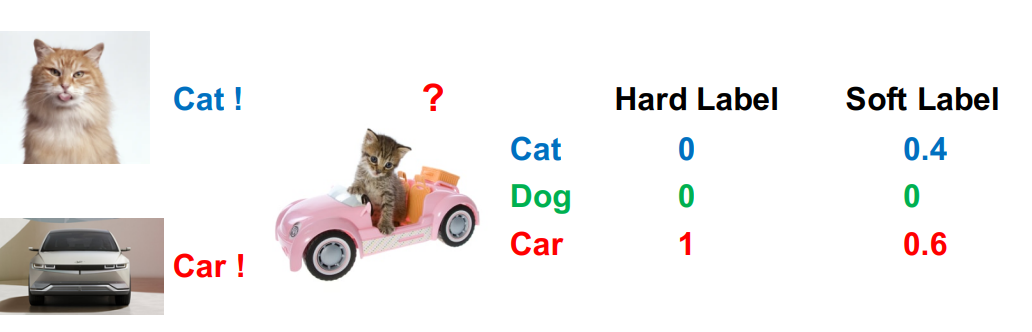
\includegraphics[scale=0.7]{2nd Scribe Notes/illustration4.PNG} \\
    
    While the cat and car are easily recognized, the third image of a cat inside a car, has quite different results between hard label and soft label.\\
    \\
    \subsection{Feature-based Knowledge:} 
    
    We can also use the data from the intermediate hidden layers in the teacher model to train the student model. An example of this techniques when used in computer vision with local structure preserving(LSP) is stated below:
    \\
    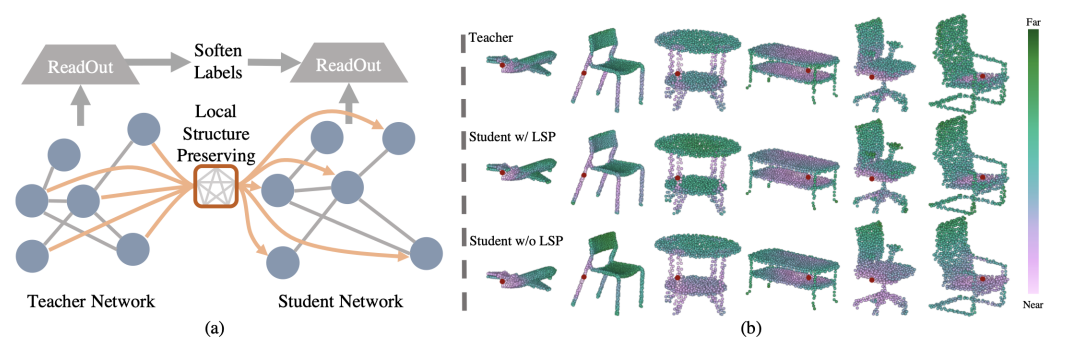
\includegraphics[scale=0.7]{2nd Scribe Notes/illustration5.PNG}
    \\    
    Acc. to Yang et al, the local structure is denoted by formula:\\
    
    $LS_{ij} = \frac{e^{{||z_i-z_j||}^2_2}}{\sum_{j:(j,i)\in \epsilon}({||z_i-z_j||}^2_2)}$ \\
    \\
    Acc. to Zhang et al(2021), we have Attention and Global Relation (C: Channel; H:
    Height; W: Width) as follows:\\

    $Attention: G^c(A) = \frac{1}{HW}\sum^H_{i=1}\sum^W_{j=1}|A_{.,i,j}|$\\
    
       $G^S(A)=\frac{1}{C} \sum^C_{i=1}|A_{i,.,}|$\\
       
       $Relation: r_{i,j} = \frac{1}{WH}\sum^H_{i'=1}\sum^W_{j'=1}f(A._{,i,j},A._{,i',j'})g(A._{,i',j'})$\\
    \\  
    This is shown to improve object detection with Feature-based Knowledge
    Distillation giving accurate and efficient detectors.
    \\
    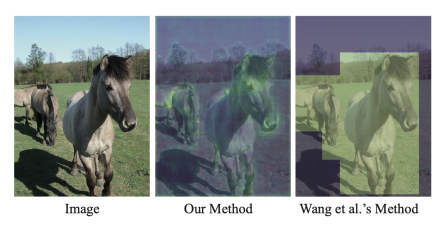
\includegraphics[scale=1.0]{2nd Scribe Notes/illustration6.PNG}
    \\
    \subsection{Relation-based Knowledge:} 
    
    In this approach, we do not evaluate the layers, but instead compare pairs of layers to find their instance relation and distill that information from teacher to student model. Here we have:\\
    
    $\pounds_{R'}(F_t,F_s) = \pounds(\phi_t(t_i,t_j),\phi_s(s_i,s_j))$\\
    \\
    where $\phi(f_i,f_j)$: Relation between $f_i$ and $f_j$ \\
    $ \pounds : l1{}norm,{} l2{} norm, {}l_{CE}$
    
    \section{Distillation Schemes}
    There are 3 types of knowledge distillation:\\
    \\
    1) Offline distillation: here we assume the teacher model is well trained and use it train student. Whatever we discussed till now was offline distillation.\\
    \\
    2) Online distillation: here we simultaneously train the teacher model and enhance the student network.\\
    \\
    3) Self distillation: here the student model teaches itself through repeated iterations of learning from itself.
    
    \section{Teacher-Student Architecture}
    There are 3 ways to choose student architecture:\\
    \\
    1) Student model is chosen from the simplified version of the teacher model. Here our aim is to preserve the features of the specific model while simplifying it.\\
    \\
    2) Smaller size of the teacher model is used as the architecture for the student model. This is represented below:
    \\
    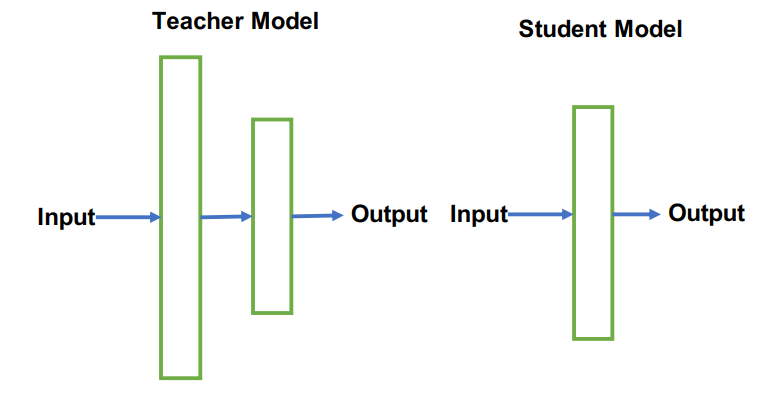
\includegraphics[scale=0.9]{2nd Scribe Notes/illustration7.PNG}
    \\
    3) Using the teacher model as the student model unchanged. In cases where we do not require a simplified version, this is chosen.
    
    \section{Why Knowledge Distillation Works}
        In the Under Parameters Regime: \\
        One hot risk: $\hat{R}(f)$ \\
        Bayes Distilled Risk: $\hat{R}_*(f)$ \\
        Overfitting is caused by low-bias and high-variance. \\
        $\mathbb{V}[\hat{R}_*(f)] \le \mathbb{V}[\hat{R}(f)]$ \\
        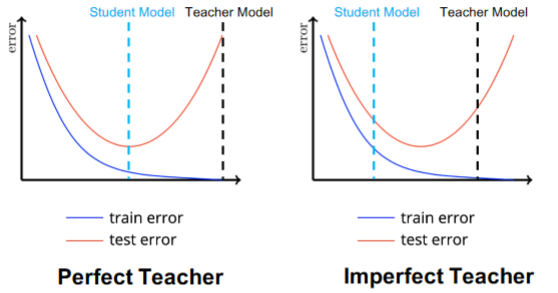
\includegraphics[scale=0.9]{2nd Scribe Notes/risk.PNG} \\
        
    \section{Generalization Bound Perspective}
        \textbf{Observation:} The Generalization bound is not good for deep models. \\
        This is because of the large  Vapnik–Chervonenkis (VC) dimension. \\
        \\
        \textbf{Distillation error:} Given a multi-class predictor $f$: $\mathbb{R}^d \rightarrow \mathbb{R}^k$ , the goal is to find another predictor $g$: $\mathbb{R}^d \rightarrow \mathbb{R}^k$ which is simpler, but still similar in distillation error $\phi_{\gamma,n}$, defined along with $\phi_\gamma$, the softmax with temperature $\gamma > 0$, as: \\
        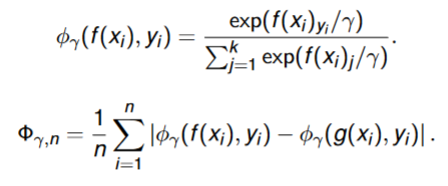
\includegraphics[scale=0.9]{2nd Scribe Notes/dist_error.png} \\
        
        The distillation process can be thought as matching the $G_j$ one by one until the distillation error is small. Then we announce that $f$ inherits the generalization properties of $G_j$. \\
        \\
        \textbf{Lemma:} With any set of multiclass predictors $G_j$ where $g\in G$, with probability at least $1-\delta$, \\
        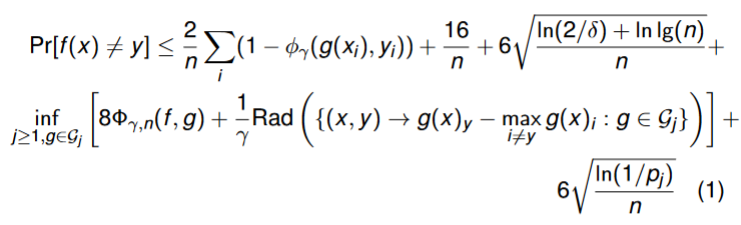
\includegraphics[scale=0.9]{2nd Scribe Notes/dist_error_2.PNG} \\
        Therefore, \\
        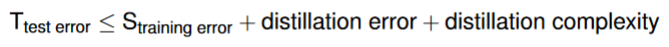
\includegraphics[scale=0.9]{2nd Scribe Notes/test_error.PNG} \\
        \\
        \section{Neural Tangent Kernel in Wide Neural Network}
        This method uses the Kernel to explain the Artificial Neural Network where the neural network can be thought of as a kernel function which maps $\mathbb{R}^d \rightarrow \mathbb{R}^k$ when $k\gg d$ \\
        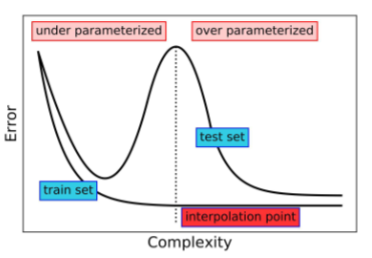
\includegraphics[scale=0.9]{2nd Scribe Notes/parameter_graph.PNG} \\
        Assume that $x$ is the input, $\theta$ is all parameters in the network, and $f(\theta, x)$ is the output of the network: \\
        $\frac{df(\theta_t, x_t)}{dt}=-H(t)*(f(\theta_t, x_t)-y)$, where the $(i, j)$-th entry of $H(t)$ is $\langle \frac{\partial f(\theta_t, x_i)}{\partial \theta}, \frac{\partial f(\theta_t, x_j)}{\partial \theta}\rangle$ \\
        \\
        Thus $H(t)$ is the kernel matrix: $ker_t(x, x')=\langle \frac{\partial f(\theta_t, x)}{\partial \theta}, \frac{\partial f(\theta_t, x')}{\partial \theta}\rangle$, $\forall x, x' \in \mathbb{R}^d$ \\
        When the width of the network is infinite, the time-varying kernel would approximate to a fixed kernel of the form: $ker(x, x')=\mathbb{E}_{\theta~w}[\langle \frac{\partial f(\theta_t, x)}{\partial \theta}, \frac{\partial f(\theta_t, x')}{\partial \theta}\rangle]$ Which is the Neural Tangent Kernel (NTK). \\
        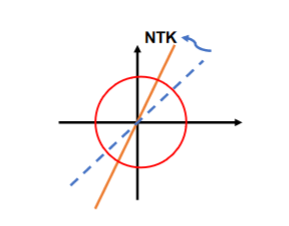
\includegraphics[scale=0.9]{2nd Scribe Notes/NTKPNG.PNG} \\
        \textbf{Theorem:} The transfer risk is bounded by: $\mathbb{R}_n\le p(\frac{\pi}{2}-\bar{\alpha}_n=\mathcal{O}(n^{-b/2})$ \\
        \\
        \section{Empirical Perspective}
        \textbf{Observation:} Knowledge Distillation and Ensemble do not aid generalization when the input is Gaussian or Gaussian-like. Consider a binary classification problem, where the data contains 4 features, $v=\{v_1,v_2,v_3,v_4,\}$ \\
        For the first label, we have: \\
        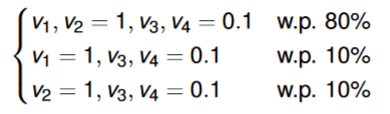
\includegraphics[scale=0.9]{2nd Scribe Notes/wp1.PNG} \\
        And for the second label, we have: \\
        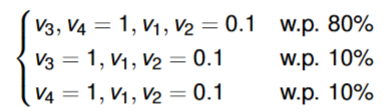
\includegraphics[scale=0.9]{2nd Scribe Notes/wp2.PNG} \\
        \\
        The training process for a single model is in two phases:
        \begin{enumerate}
            \item{The network will quickly pick up one of the features $v\in\{v_1,v_2\}$ for the first label, and one of the features $v'\in\{v_3,v_4\}$ for the second label}
            \item{The network will memorize the remaining $10\%$ of the training examples without learning any new features}
        \end{enumerate}
        Single Model: $100\%$ training accuracy, $90\%$ testing accuracy. \\
        $v_1, v_2$: first label. $v_3, v_4$: second label \\
        \textbf{Conclusion:} Knowledge Distillation forces the model to learn every feature of the label.
\end{document}

    
    

